\documentclass[]{article}
\usepackage[a4paper, total={7in, 8in}]{geometry}
\usepackage{apacite}

%opening
\title{Simulation results of Population Receptive Field response with \\ Compressive Spatial Summation model}
\author{Arash Ashrafnejad}

\usepackage{graphicx}
\usepackage{float}

\begin{document}

\null  % Empty line
\nointerlineskip  % No skip for prev line
\vfill
\let\snewpage \newpage
\let\newpage \relax
\maketitle
\let \newpage \snewpage
\vfill 
\break % page break


\section{Introduction}

A population receptive field (pRF) is the region of the visual field where stimuli illicit responses from a local population of neurons. In \cite{Dumoulin2008} the authors proposed a model of neuronal population receptive field defined by a two-dimensional Gaussian function:

\begin{equation}
	g(x, y) = e^{-\frac{(x-x_0)^2+(y-y_0)^2}{2\sigma^2}}
\end{equation}

Recent study by \cite{Kay2013} showed that linear spatial summation model proposed by \shortcite{Dumoulin2008} deviates from linearity in early visual areas (e.g., V1, V2) and grows more in the anterior extrastriate areas (e.g., LO-2, VO-2) and the data is more accurately explained when this compressive static nonlinearity is applied after linear summation.

According to the Compressive Spatial Summation (CSS) model proposed by \shortcite{Kay2013}, the pRF response is modeled as the element-wise (Hadamard) product of effective stimulus $s(x, y, t)$ and the Gaussian pRF model $g(x, y)$ then raised to power $n$ and multiplied with a gain factor $g$.
\begin{equation}
	r(t) = g (\sum_{x, y} s(x, y, t) g(x, t))^n
\end{equation}

\section{Results}
In an attempt to evaluate the CSS model as the underlying assumed model for simulation, we have used different exponent values from 0.5 to 1.0 with no gain.

The voxel-wise simulated $x$, $y$ and $\sigma$ estimation error percentages corresponding to the stimuli visual field for each exponent value is obtained as plotted in Figures 1 to 6.

\section{Discussion and Conclusion}
From Figures 1 and 6 we see that the average errors decrease when we apply static compressive nonlinearity upto $n=0.6$.

The reason for this can be seen from the error map of individual voxels. As n decreases (i.e., more spatial compressing) the receptive field away from the fixation point become easier to estimate (i.e., lower estimation error) which means they become more responsive to the stimuli.

However, with more spatial comprression the noise also gets amplified and eventually the average errors increase as shown from Figures 5 and 6. Therefore, there is a trade-off and an optimal exponent value which gives the highest average estimation power over all voxels.

Since it is shown by \shortcite{Kay2013} that exponent values are decreasing from unit value (i.e., increased spatial nonlinearity) for early to higher visual field areas, we can simulate these areas more realistically by using CSS pRF response model. Furthermore, our simulation results can simulate the signal-to-noise ratios of different visual areas based on these empirical exponent values.
\bibliographystyle{apacite}
\bibliography{refs}



\begin{figure}[htp]
	\centering
	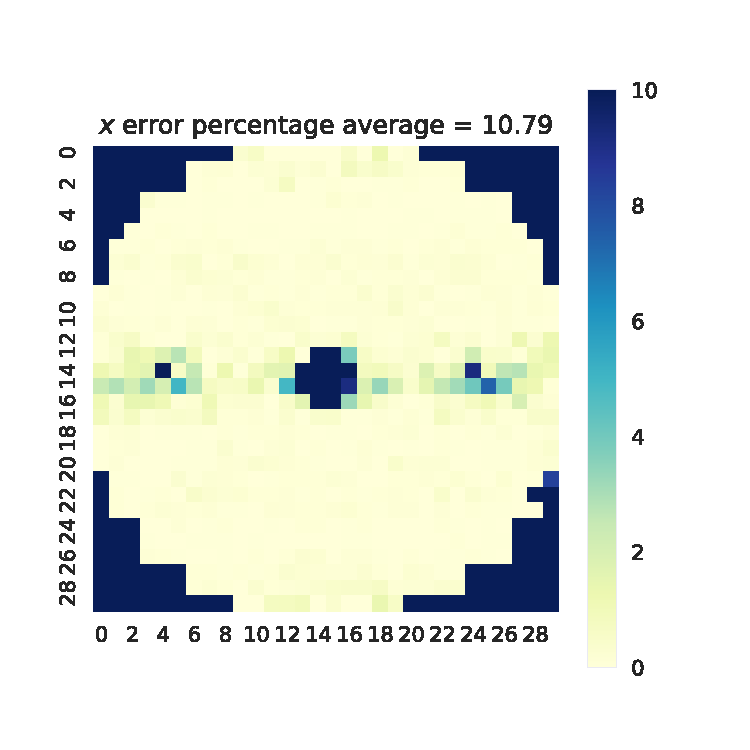
\includegraphics[width=.32\textwidth]{x_10}
	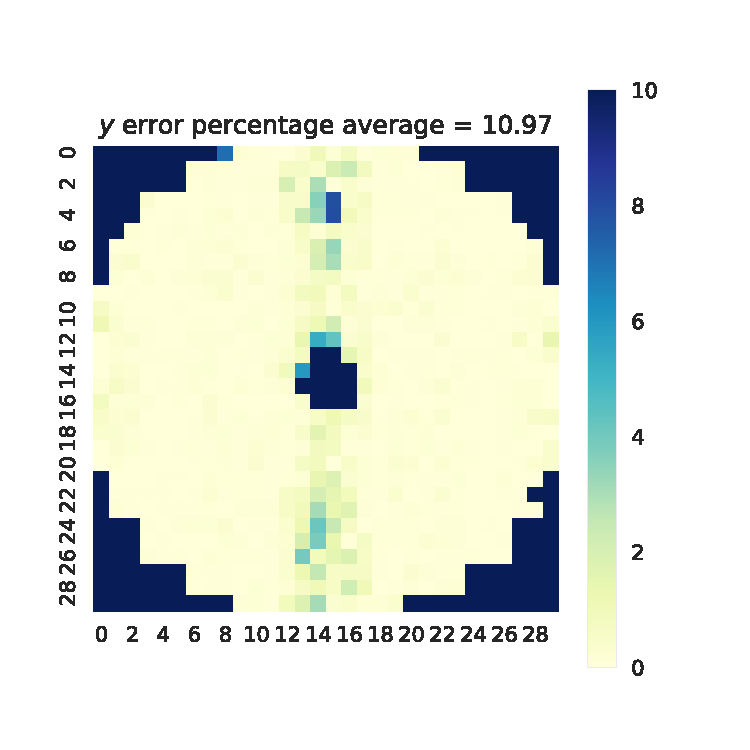
\includegraphics[width=.32\textwidth]{y_10}
	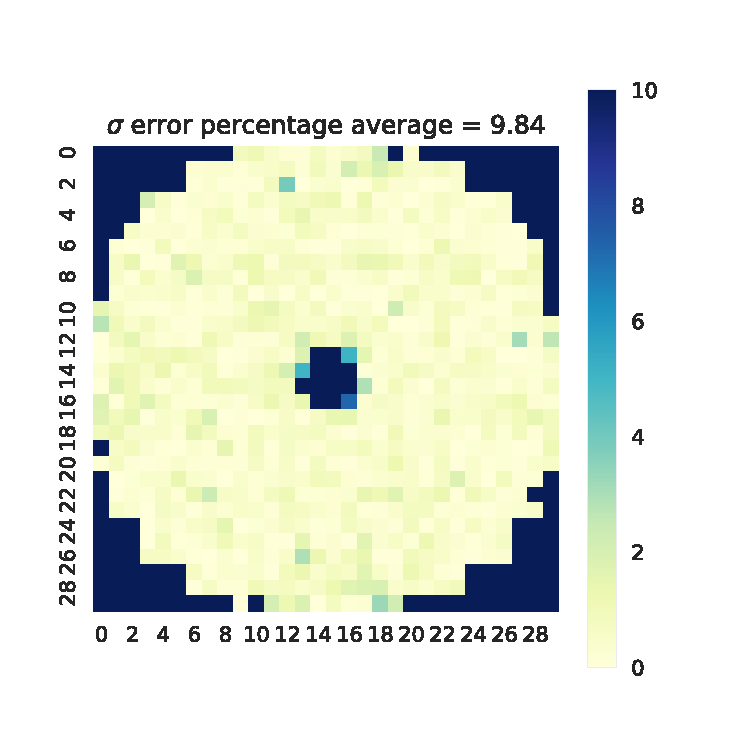
\includegraphics[width=.32\textwidth]{sigma_10}
	\vspace{-0.5cm}
	\caption{Linear model with $n=1.0$}
	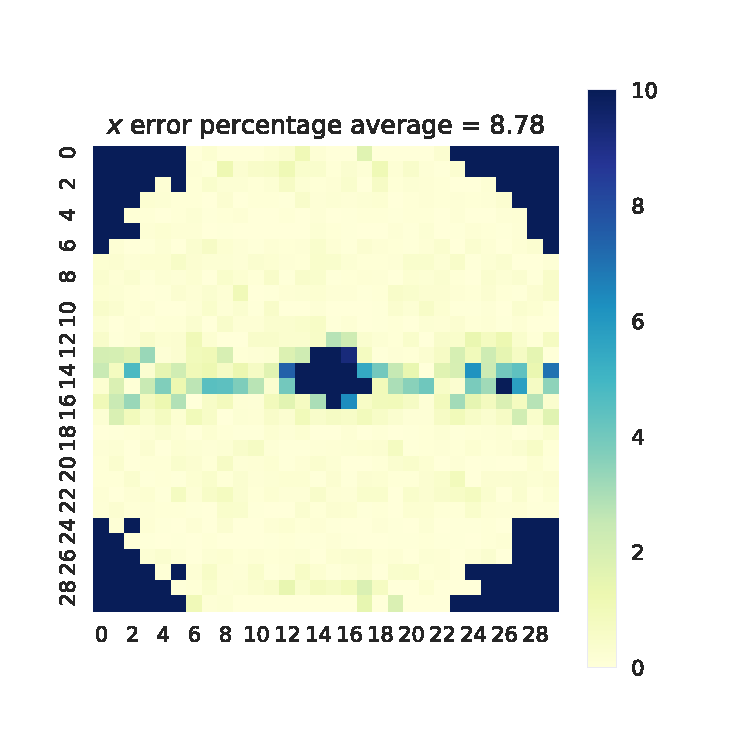
\includegraphics[width=.32\textwidth]{x_9}
	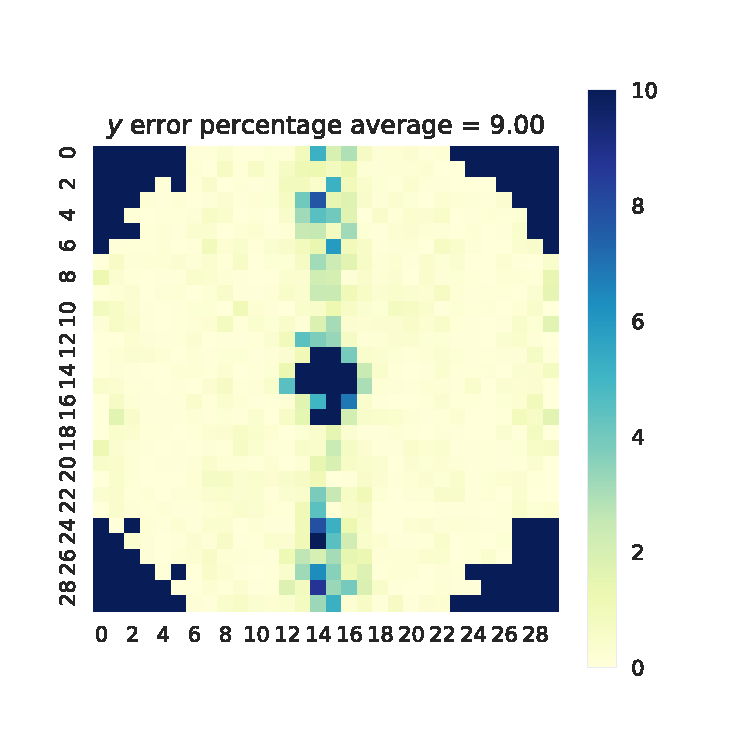
\includegraphics[width=.32\textwidth]{y_9}
	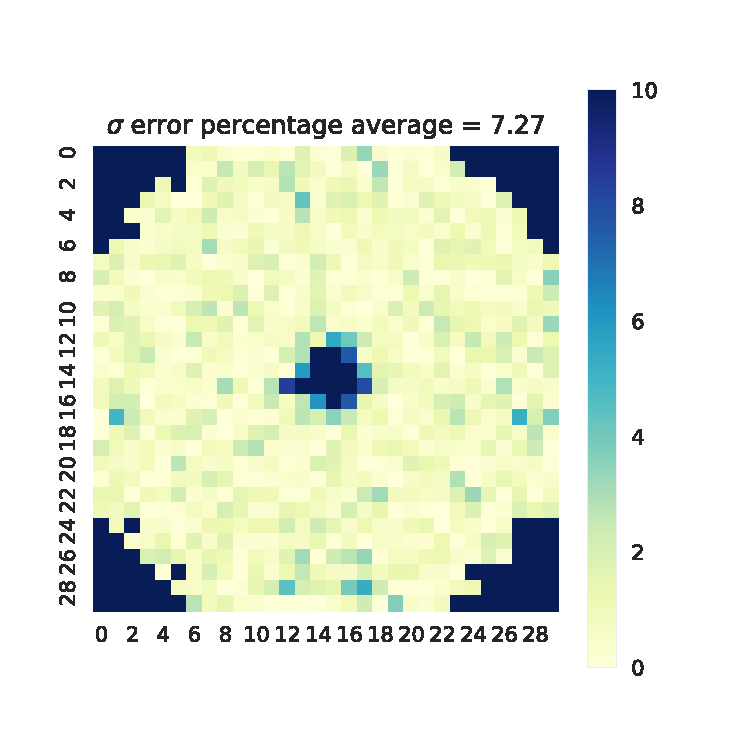
\includegraphics[width=.32\textwidth]{sigma_9}
	\vspace{-0.5cm}
	\caption{CSS model with exponent $n=0.9$}
	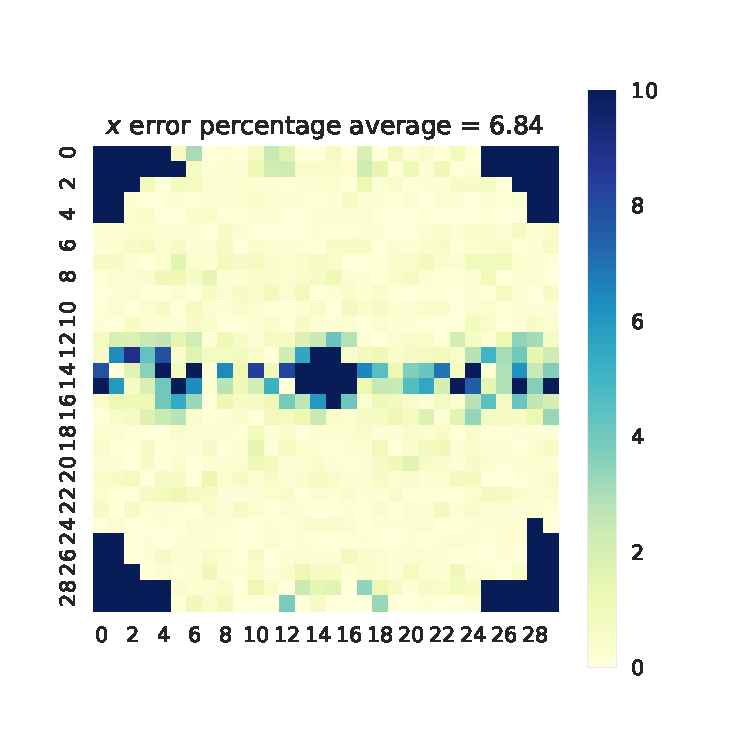
\includegraphics[width=.32\textwidth]{x_8}
	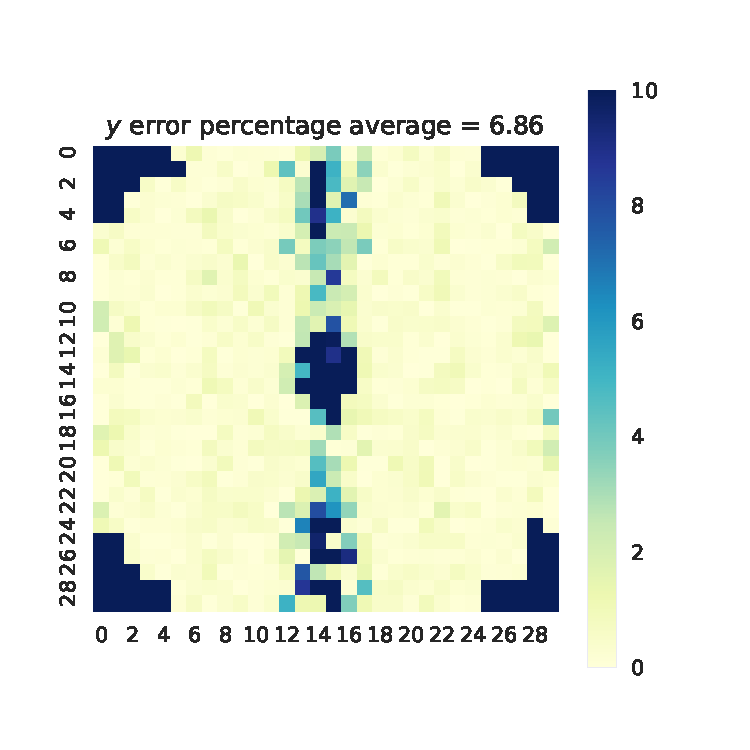
\includegraphics[width=.32\textwidth]{y_8}
	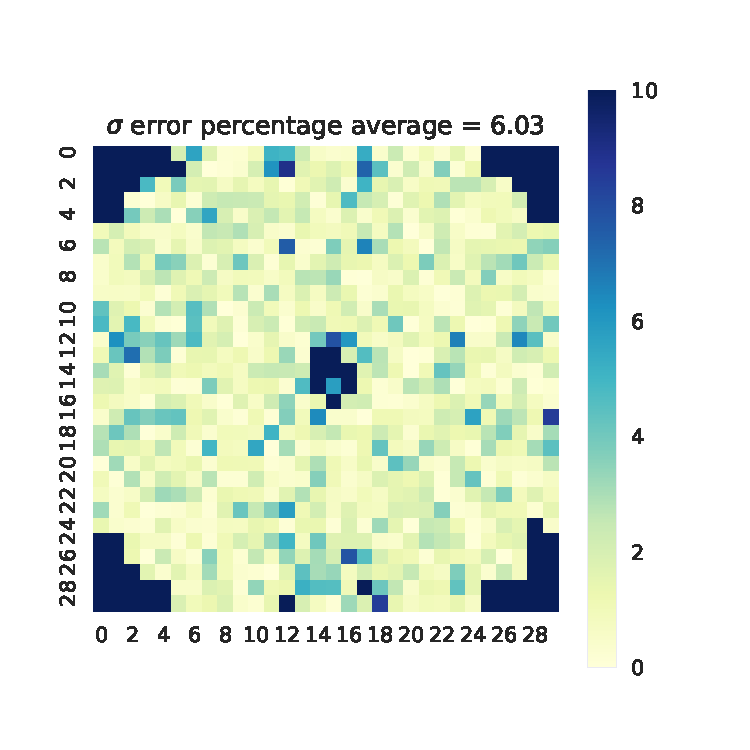
\includegraphics[width=.32\textwidth]{sigma_8}
	\vspace{-0.5cm}
	\caption{CSS model with exponent $n=0.8$}
\end{figure}
\begin{figure}[htp]
	\centering
	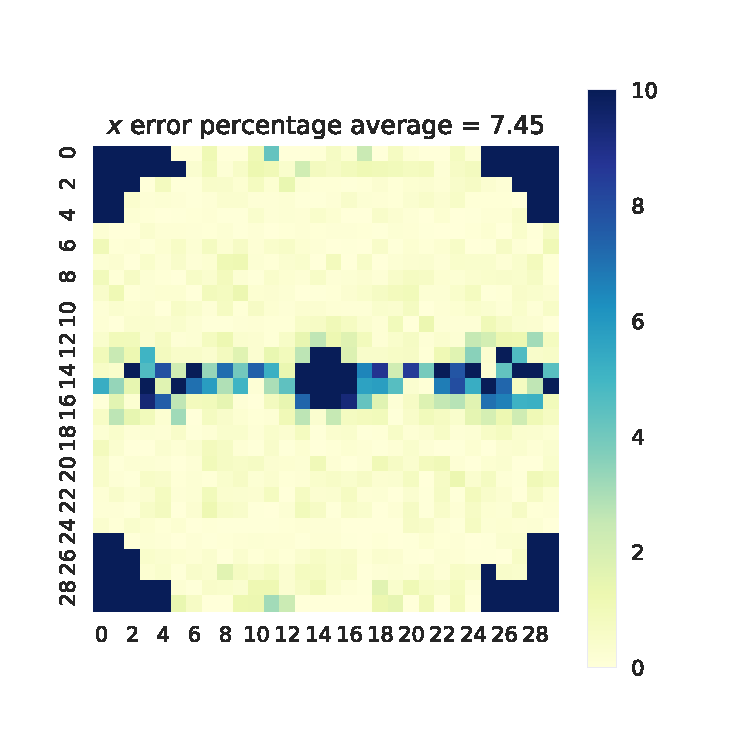
\includegraphics[width=.32\textwidth]{x_7}
	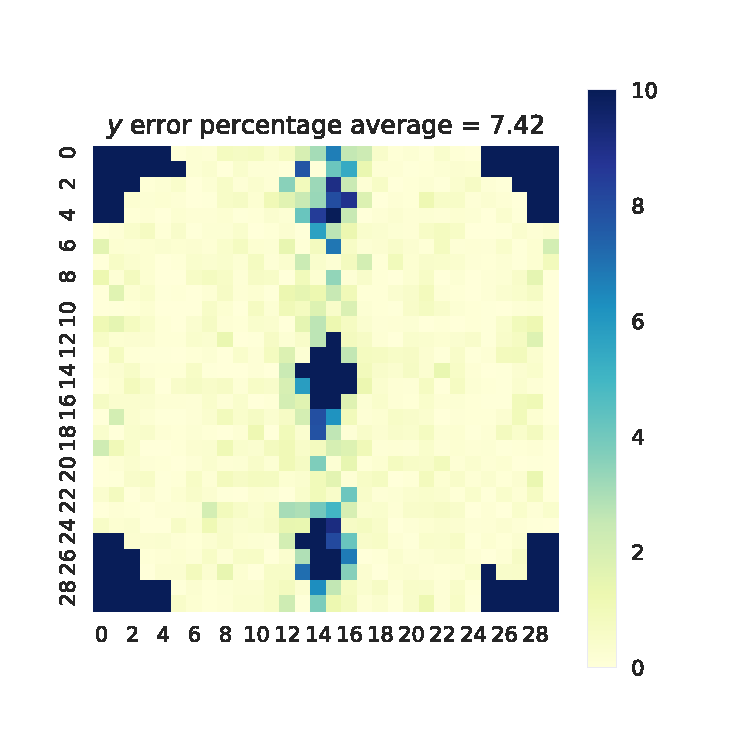
\includegraphics[width=.32\textwidth]{y_7}
	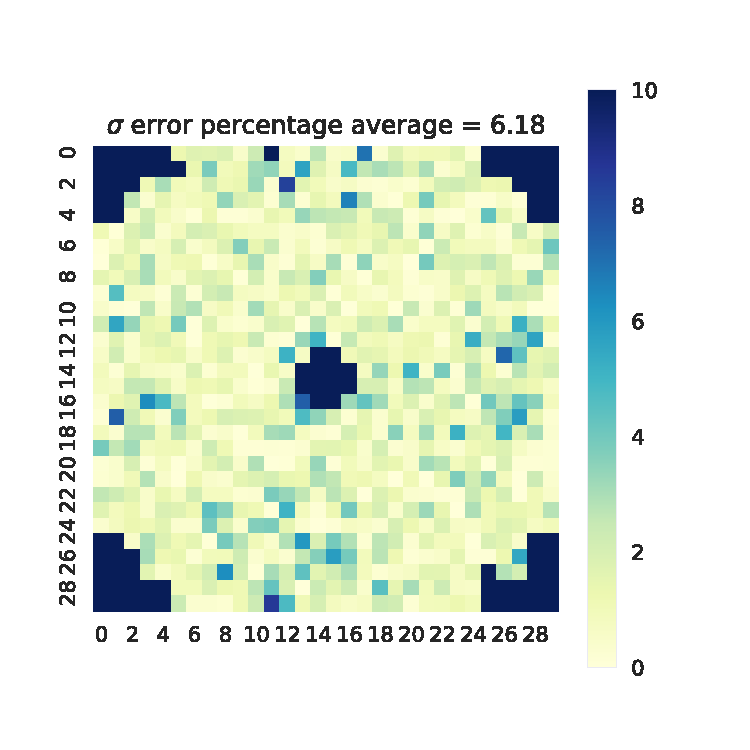
\includegraphics[width=.32\textwidth]{sigma_7}
	\vspace{-0.5cm}
	\caption{CSS model with exponent $n=0.7$}
		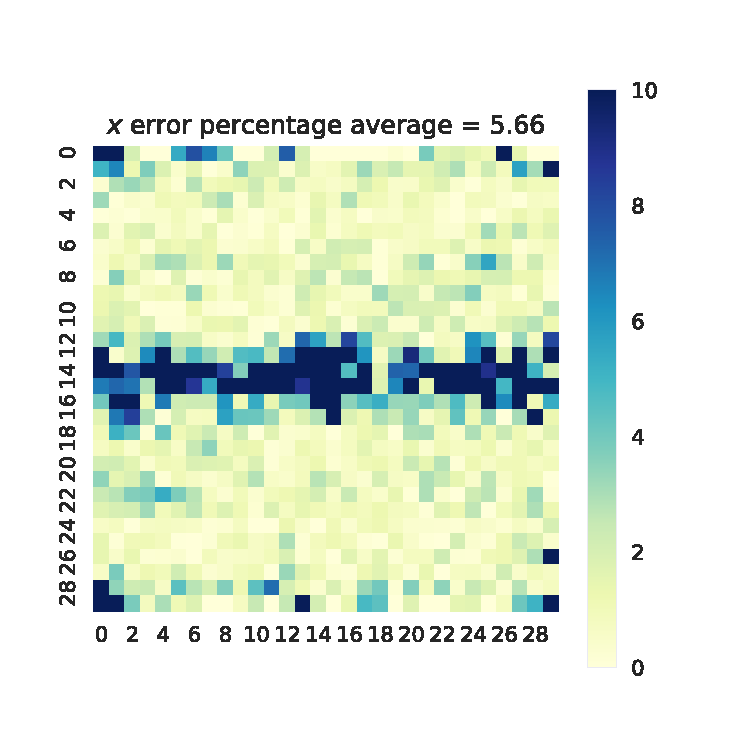
\includegraphics[width=.32\textwidth]{x_6}
	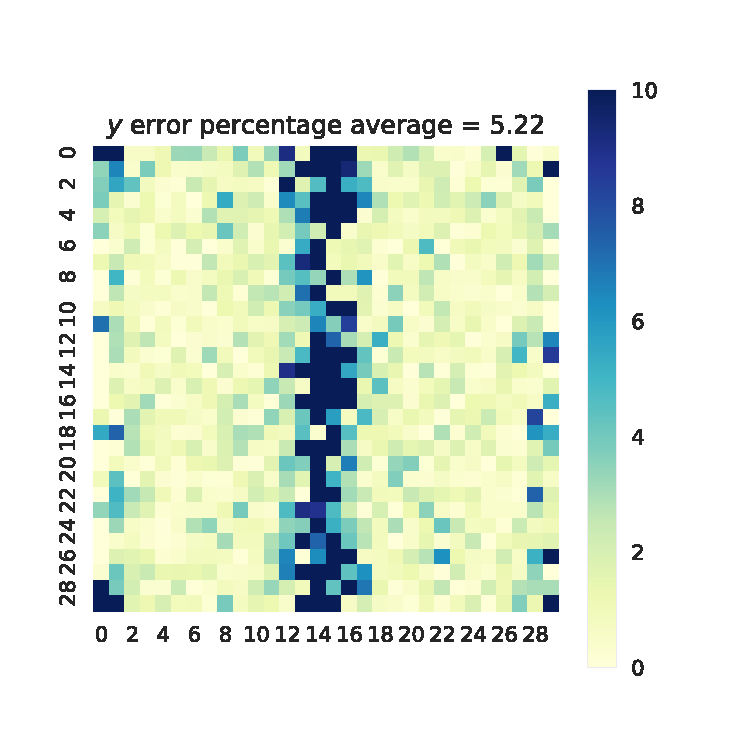
\includegraphics[width=.32\textwidth]{y_6}
	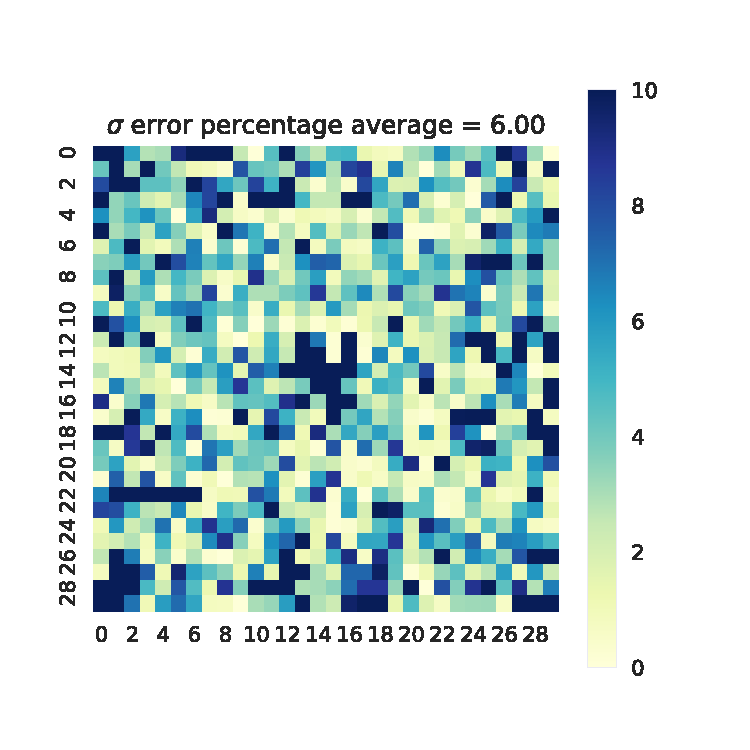
\includegraphics[width=.32\textwidth]{sigma_6}
	\vspace{-0.5cm}
	\caption{CSS model with exponent $n=0.6$}
	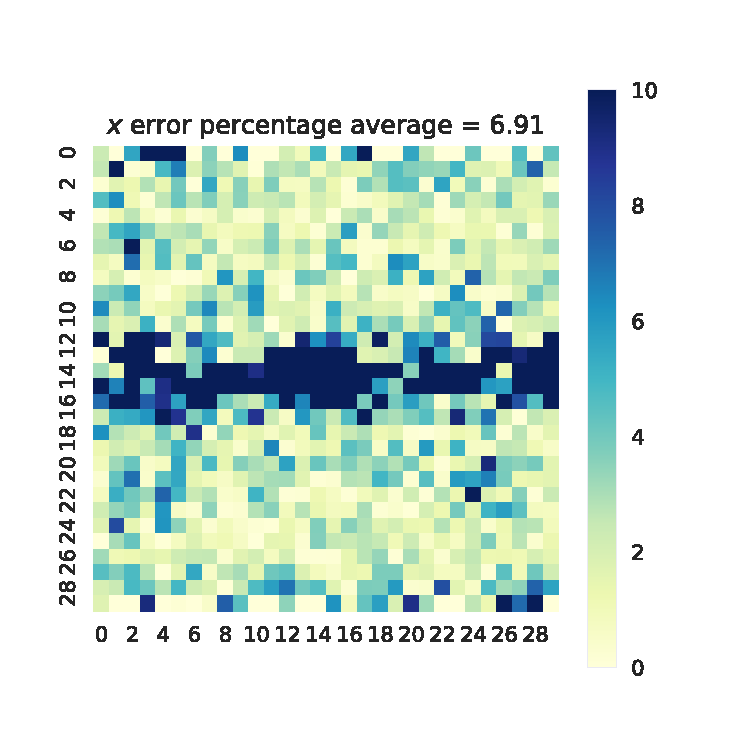
\includegraphics[width=.32\textwidth]{x_5}
	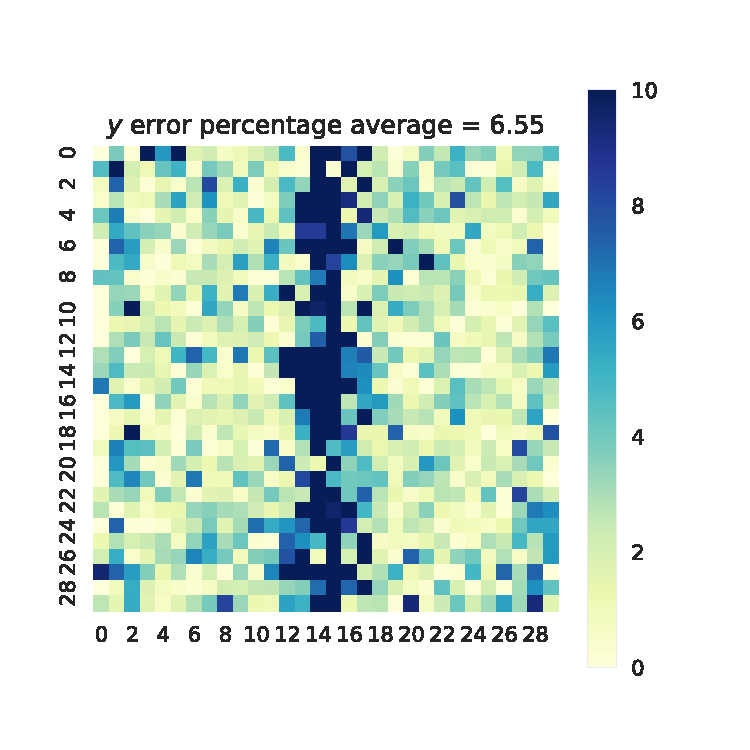
\includegraphics[width=.32\textwidth]{y_5}
	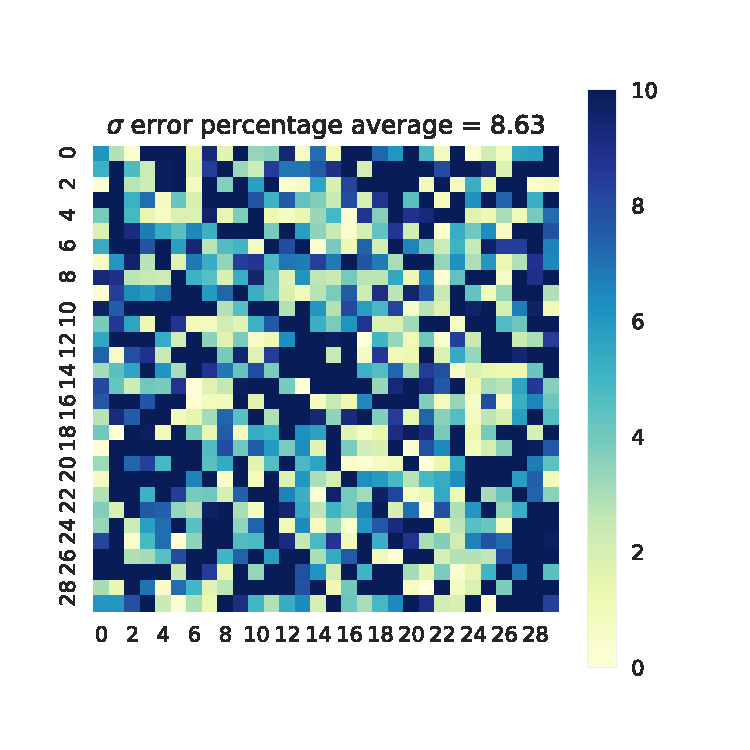
\includegraphics[width=.32\textwidth]{sigma_5}
	\vspace{-0.5cm}
	\caption{CSS model with exponent $n=0.5$}
\end{figure}




\end{document}
